\documentclass[12pt,a4paper]{article}

\usepackage[T1]{fontenc}
\usepackage[utf8]{inputenc}
\usepackage[english]{babel}
\usepackage{amsmath,amssymb}
\usepackage{setspace}
\usepackage{booktabs}
\usepackage{array}
\usepackage{graphicx}
\usepackage{caption}
\usepackage{titlesec}
\usepackage{enumitem}
\usepackage[margin=1in]{geometry}
\usepackage[hidelinks]{hyperref}
\usepackage{xcolor}
\graphicspath{{../figures/report_en/}{figures/report_en/}{../figures/}{figures/}}

% ---- Section style: Roman sections, alphabetic subsections (author's house style) ----
\renewcommand{\thesection}{\Roman{section}.}
\renewcommand{\thesubsection}{\Alph{subsection}.}
\titleformat{\section}{\normalfont\large\bfseries}{\thesection}{0.7em}{}
\titleformat{\subsection}{\normalfont\normalsize\bfseries}{\thesubsection}{0.7em}{}
\titlespacing*{\section}{0pt}{1.6\baselineskip}{0.6\baselineskip}
\titlespacing*{\subsection}{0pt}{1.1\baselineskip}{0.4\baselineskip}

% ---- Table-note command (author's house style) ----
\newcommand{\tnote}[1]{\par\vspace{1.2ex}\begin{spacing}{1.0}\small\noindent #1\par\end{spacing}\vspace{1.2ex}}

% ---- Citation footnote helper: sources are cited in footnotes ----
\newcommand{\cf}[1]{\footnote{#1}}

\setlength{\parindent}{1.5em}

\begin{document}

%============================ TITLE PAGE ============================
\thispagestyle{empty}
\begin{center}
\vspace*{2.3cm}
{\fontsize{17}{21}\selectfont Realized-Volatility Forecasting and Volatility-Managed Sizing on the S\&P~500}\\[0.5cm]
{\fontsize{14}{18}\selectfont A Pre-Registered, Walk-Forward,\\[2mm]
Multiple-Testing-Corrected Study --- with an Honest Null}\\[1.8cm]
{\normalsize JONAS L\"OFFLER\renewcommand{\thefootnote}{$*$}\footnote{Independent researcher
(contact via the repository issue tracker). Code, the pre-registration protocol and the full result tables
are provided in the accompanying repository; licensed raw data are not redistributed (sha256
fingerprints published). Research and educational project, not investment advice. All results are
out-of-sample and, unless stated otherwise, net of assumed transaction costs on a price index.
All numbers reproduce deterministically from the versioned code (seed~42) and the author bears full
substantive responsibility.}}\\[0.9cm]
{\normalsize \today}\\[1.7cm]
{\normalsize\textbf{\textsc{Abstract}}}
\end{center}

\begin{spacing}{1.0}
\begin{quote}\small
\hspace{1.5em}We study realized-volatility forecasting and volatility-managed exposure sizing on
21~years of one-minute S\&P~500 data, conditioned on the VIX term structure, under a validation
protocol fixed \emph{before the first run}: pre-registered hypotheses, grids, costs and ranking
rule; walk-forward parameter selection on training windows only; and multiple-testing corrections
across the 73~configurations actually computed. Two results emerge, of opposite sign.
\emph{Forecasting holds up:} log-HAR attains a lower out-of-sample QLIKE than the random walk, and
a nested mean-squared-prediction-error Clark-West test rejects equal accuracy ($p\approx0.03$); the
edge grows with horizon (MSE-based $R^2_{OOS}$ from $+23\,\%$ at $h{=}1$ to $+43\,\%$ at $h{=}22$),
implied volatility adds information (HAR-IV, $p=0.019$), and a rich linear feature set edges HAR-IV
through \emph{features} rather than regularization or nonlinearity. A loss-matched Gamma-GLM with
the VIX term-structure slope is the strongest of a few candidates to lower \emph{both} QLIKE ($-4\,\%$) and MSE, in
both sub-periods (Diebold-Mariano $p=0.0008$, exploratory). A lag diagnostic shows the forecast is
well calibrated on average (Mincer-Zarnowitz slope $\approx1$, top-forecast-decile ratio~1.08, tail
coverage~$9.8\,\%$); its visible ``lag'' is largely mechanical --- of the $2.54\times$
spike-underestimation a perfectly-calibrated forecaster already produces $\approx1.90\times$, and
only the residual ($+0.64$, $P<0.001$) is genuine under-reaction to unanticipated shocks.
\emph{The trading strategy does not hold up:} the best walk-forward volatility-managed /
VIX-term-structure combination (Sharpe~0.96, maximum drawdown $-9.9\,\%$ versus buy-and-hold
$0.83\,/\,{-}34.0\,\%$) is \emph{disqualified by the study's own pre-registered rules} --- probability
of backtest overfitting~0.84 and a single-market effect --- its Sharpe advantage lies inside the
bootstrap noise band, and its clean drawdown profile is largely a volatility-level artifact. Every
failure is reported. The contribution is the forecasting result and the validation methodology, not
a tradeable edge; no result reaches \texttt{supported} status without a live prediction log.
\end{quote}

\vspace{0.4cm}
\noindent\small\textit{Keywords:} realized volatility, HAR, volatility-managed portfolios, VIX term
structure, walk-forward analysis, backtest overfitting, deflated Sharpe ratio, null result.\\
\textit{JEL:} C22, C53, C58, G11, G17.
\end{spacing}

\newpage
\setcounter{page}{1}
\setcounter{footnote}{0}
\renewcommand{\thefootnote}{\arabic{footnote}}
\doublespacing

%============================ I. INTRODUCTION ============================
\section{Introduction}

Two empirical regularities motivate the study. First, \emph{volatility is forecastable and returns
are barely so}: realized variance has strong, slowly-decaying autocorrelation, whereas daily index
returns are close to unpredictable.\cf{Andersen, Bollerslev, Diebold \& Labys (2003); Corsi (2009).}
Second, \emph{the reward-to-risk of equity exposure is not constant}, so scaling exposure inversely
to expected volatility can raise risk-adjusted performance\cf{Moreira \& Muir (2017).} --- though
this result is fragile out of sample.\cf{Cederburg, O'Doherty, Wang \& Yan (2020).}

This paper is deliberately a methodology paper with an honest outcome. Its value is not a headline
Sharpe but the discipline applied to a practical question, and the willingness to report --- and
\emph{act on} --- a null. The design rests on four commitments. (i)~\emph{Pre-registration:}
hypotheses (with null and expected effect), the complete grids, the cost model, the out-of-sample
split, and the ranking and disqualification rules were fixed in writing before the first campaign
backtest. (ii)~\emph{Walk-forward everywhere:} no reported strategy uses parameters chosen on the
data it is evaluated on; parameters are re-selected annually on trailing windows. (iii)~\emph{Multiple-testing
accounting:} every configuration computed ($n=73$) enters the deflated Sharpe correction, and the
combination universe is additionally audited with the probability of backtest overfitting via
combinatorially symmetric cross-validation.\cf{Bailey \& L\'opez de Prado (2014); Bailey, Borwein,
L\'opez de Prado \& Zhu (2017).} (iv)~\emph{Full reporting, including disqualification:} when the
study's own rules disqualify its best strategy, that becomes the result.

\emph{Scope.} We publish the S\&P complex only (SPX~+~VIX) --- the data whose provenance we fully
stand behind. This choice interacts with the pre-registration in a way that is central to the paper:
the fixed rules \emph{disqualify single-market-only effects}, so a single-market strategy result
\emph{cannot} be a tradeable claim by the study's own ex-ante standard. That is not a limitation
worked around; it is the honest conclusion. The replication literature warns repeatedly how easily
backtest ``edges'' arise from multiple testing and selective reporting,\cf{White (2000); Harvey, Liu
\& Zhu (2016); Bailey, Borwein, L\'opez de Prado \& Zhu (2014).} and the present protocol is built to
disqualify its own favourite result rather than to survive review.

The remainder is organized as follows. Section~II describes the data and realized measures;
Section~III the forecasting layer; Section~IV the lag diagnostics that decompose the apparent
forecast ``lag''; Section~V the strategy design and validation protocol; Section~VI the disqualified
campaign; Section~VII implementation and costs; Section~VIII a deliberately sharp self-assessment;
and Section~IX concludes.

\begin{figure}[t]\centering
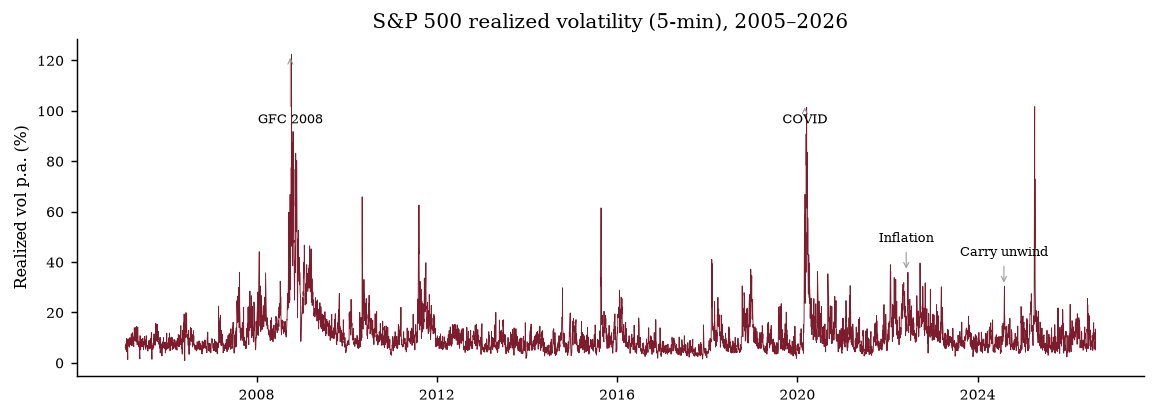
\includegraphics[width=\linewidth]{01_rv_history.png}
\caption{Annualized realized volatility of the S\&P~500 from five-minute returns, 2005--2026.
Volatility clusters and mean-reverts slowly --- the raw material of the forecasting result.}
\label{fig:rvhist}
\end{figure}

%============================ II. DATA ============================
\section{Data and Realized Measures}

\emph{Intraday.} Licensed one-minute index candles (MarketTick) for the S\&P~500, February~2005 to
August~2026, regular trading hours (index prints, not exchange trades --- the S\&P~500 cash index is
not itself tradeable); $5{,}543$ daily session files, of which $5{,}417$ enter the modelling panel
after HAR warm-up and VIX alignment. The raw feed also carries roughly one hundred weekend-dated
vendor files, all excluded by the trading-day and VIX alignment --- the panel contains zero weekend
dates; the out-of-sample window holds $3{,}422$ trading days. Daily realized measures are built from
five-minute sampling (realized variance, bipower variation, jumps, semivariances, realized
quarticity),\cf{Andersen, Bollerslev, Diebold \& Labys (2003); Barndorff-Nielsen \& Shephard (2004).}
which is the standard microstructure-noise/efficiency compromise.\cf{Liu, Patton \& Sheppard (2015).}

\emph{Volatility term structure.} Two distinct sources. The VIX \emph{level} used by HAR-IV
($\mathrm{ivar}=(\mathrm{VIX}/100)^2/252$) is daily-sampled from the \textbf{licensed MarketTick
one-minute VIX feed} (\texttt{data/raw/vix}, a separate licensed feed of ${\sim}5{,}280$ daily
files), \emph{not} FRED; only the term-structure slope $\ln(\mathrm{VIX3M}/\mathrm{VIX})$ is from
FRED (\texttt{VXVCLS}, \texttt{VIXCLS}). Both are re-indexed to trading days, forward-filled at most
five days, and lagged one day wherever used; reproducing the ladder from HAR-IV downward requires
the MarketTick VIX feed, not FRED alone.

\emph{Conventions.} (i)~The S\&P~500 is used as a price index: long-only CAGRs are understated by
roughly the dividend yield; all candidates share the bias. (ii)~The out-of-sample period runs from
2~January 2013; 2008 lies in the training region only. (iii)~Weights for day~$t$ use information to
the close of $t-1$, enforced by lagging every signal; an automated look-ahead test guards the
pipeline. (iv)~The risk-free rate is set to zero and declared explicitly: Sharpe ratios are excess
over zero and uninvested capital is unremunerated, applied uniformly to every sleeve and to
buy-and-hold. (v)~The cost model charges one basis point per unit of turnover, stress-tested at two
and five basis points; overnight positions pay $2\,\text{bp}\times|w|$ per day; leverage is capped at
three.

\begin{figure}[t]\centering
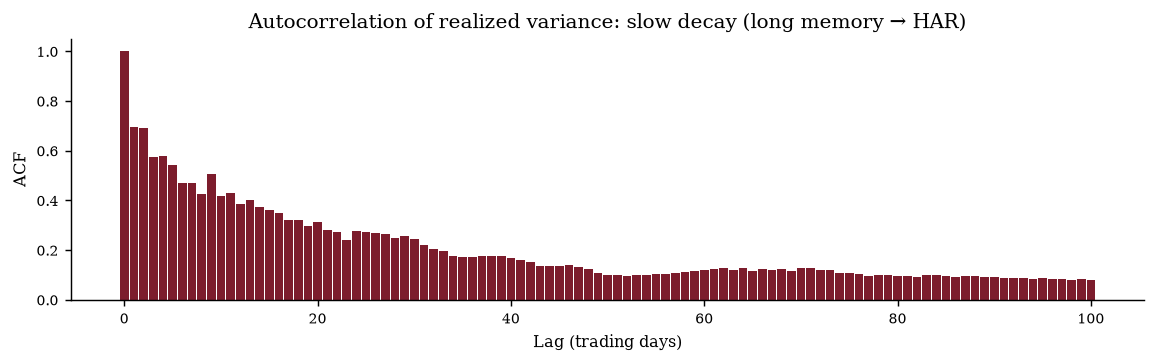
\includegraphics[width=\linewidth]{03_rv_acf.png}
\caption{The autocorrelation of daily realized variance decays roughly hyperbolically --- the
long-memory signature the HAR model captures.}
\label{fig:acf}
\end{figure}

%============================ III. FORECASTING ============================
\section{The Forecasting Layer (the result that holds)}

We evaluate a model ladder in an expanding-window out-of-sample harness (first forecast 2~January
2013, $3{,}422$ days) under QLIKE loss, which is robust to noisy volatility proxies,\cf{Patton
(2011).} with Diebold-Mariano tests\cf{Diebold \& Mariano (1995).} and, for nested comparisons,
Clark-West.\cf{Clark \& West (2007).} The Clark-West statistic is computed on squared error (MSPE),
the loss for which it is derived; QLIKE is reported separately as the ranking loss. The $R^2$ column
of Table~1 is the familiar MSE-based out-of-sample $R^2$
($1-\sum\mathrm{SE}_{\text{model}}/\sum\mathrm{SE}_{\text{RW}}$), which need not track the QLIKE
ranking.

\begin{table}[t]\centering
\textbf{Table 1. Forecast ladder --- S\&P~500, $h=1$, out-of-sample 2013--2026}
\tnote{QLIKE is the primary loss (lower is better); the $R^2$ column is the MSE-based out-of-sample
$R^2$ relative to the random walk. Dashes mark values not computed for that model. All models run
through the same expanding-window harness.}
\begin{spacing}{1.0}
\begin{tabular}{lrr}
\toprule
Model & QLIKE~$\downarrow$ & $R^2_{OOS}$ (MSE) \\
\midrule
Random walk (RV)              & 0.308 & \phantom{$+$}0\,\% \\
EWMA ($\lambda=0.94$)         & 0.351 & $-20\,\%$ \\
HAR                           & 0.247 & $+20\,\%$ \\
\textbf{log-HAR}              & \textbf{0.225} & $\mathbf{+23\,\%}$ \\
HAR-IV ($+$VIX)               & 0.204 & $+30\,\%$ \\
OLS\,/\,Ridge (rich features) & \textbf{0.197} & --- \\
Lasso\,/\,ElasticNet          & 0.198 & --- \\
Gradient boosting             & 0.205 & --- \\
\bottomrule
\end{tabular}
\end{spacing}
\label{tab:ladder}
\end{table}

Six findings follow, all from the tracked result files.

\emph{(a) log-HAR beats the random walk} --- QLIKE 0.225 versus 0.308, with a nested-MSPE Clark-West
$p\approx0.03$, the pre-registered confirmatory result.\cf{Pre-registered in
\texttt{PREREGISTRATION-FORECAST-EN.md} (vault note QR002, frozen 2026-08-15): the single
confirmatory hypothesis is QLIKE(log-HAR) $<$ QLIKE(RW) on SPX / $h{=}1$ with Clark-West $p<0.05$.
Everything else in §III is exploratory.} The $p$-value is modest relative to the loss
gap because the loss differences are heavy-tailed: a handful of spike days dominate their variance,
so the mean reduction is large but the $t$-statistic is only about~1.9. The edge grows with horizon
(MSE-based $R^2_{OOS}$ $+23\,\%$ at $h{=}1$, $+27\,\%$ at $h{=}5$, $+43\,\%$ at $h{=}22$).

\emph{(b) Implied volatility carries incremental information.} HAR-IV improves on log-HAR
(Clark-West $p=0.019$), consistent in both sub-periods.

\emph{(c) The linear feature set does the work, not regularization or nonlinearity.} Unregularized
OLS reaches QLIKE 0.1968, matching Ridge (0.1968); Lasso and ElasticNet (0.1977/0.1978) are a
statistical tie --- we do not test these fourth-decimal differences (no Model Confidence Set here;
see Section~IX), so we read the linear family as a single plateau. All beat HAR-IV (Diebold-Mariano
$p\approx0.0003$--$0.0008$), while gradient boosting adds nothing (0.2045, $p=0.86$). The honest
reading: a rich realized-feature set helps slightly; the machinery does not. The QLIKE win does not
carry to MSE, and unevenly so: the MSE-based $R^2$ is $-9.7\,\%$ for OLS and $-11.4\,\%$ for Ridge
but $-65\,\%$ for Lasso/ElasticNet, while gradient boosting (which adds nothing on QLIKE) has the
\emph{best} MSE-$R^2$ of the ladder ($+33.5\,\%$). We therefore treat the linear-feature edge as
fragile and do not build the sizing rule on it.

\emph{(d) Daily-return GARCH cannot match the random walk} once intraday RV is available (QLIKE
0.456),\cf{Bollerslev (1986); the textbook result is due to Andersen, Bollerslev, Diebold \& Labys
(2003).} confirming that intraday information dominates daily-return conditional-variance models.

\emph{(e) A multiplicity-aware check (Model Confidence Set).} To hold the forecasting layer to the
same standard as the strategy, we compute a Model Confidence Set\cf{Hansen, Lunde \& Nason (2011).}
(QLIKE loss, stationary block bootstrap, $1{,}000$ replications, block~10, seed~42) over the ten
classical ladder models $\{$RW, EWMA, AR(1), HAR, HAR-CJ, HAR-RS, HARQ, LHAR, log-HAR, HAR-IV$\}$.
The $90\,\%$ MCS is $\{$HAR-IV$\}$ alone --- every simpler model is excluded at $p<0.01$, so HAR-IV
is the unambiguous \emph{classical} winner. Admitting the rich-feature/ML models widens the set: the
$90\,\%$ MCS \emph{appears} to widen to $\{$Lasso, ElasticNet, HAR-CJ$\}$ with \textbf{HAR-IV excluded at $p=0.013$} --- but this second run is computed on a \emph{different} loss matrix (the unfiltered \texttt{loss\_matrix\_classical}, on which the same model names carry different QLIKE: HAR-CJ 0.564 vs.\ 0.256, LHAR 1.852 vs.\ 0.684), so the two MCS statements are not directly comparable. That run is moreover \emph{degenerate}: HAR-CJ (QLIKE 0.564, second-worst) sits inside the set while HAR-IV (0.204, third-best) is outside --- an unstable MCS on this matrix, not a genuine displacement (on the unfiltered matrix without the ML columns the $90\,\%$ set is simply $\{$HAR-IV$\}$). We therefore do not read it as the feature family displacing HAR-IV, and do not build the sizing rule on it, both because that QLIKE win rides the $-65\,\%$ MSE-$R^2$ of Lasso~(c) and because the comparison is not apples-to-apples.

\emph{(f) The one genuinely new candidate: a QLIKE-native GLM with the VIX term-structure slope.}
Adding the log VIX3M/VIX slope to HAR-IV and fitting it with a Gamma-GLM (log link) --- that is,
estimating \emph{in the loss the model is judged by} rather than least squares on log-RV followed by
a retransform --- reaches QLIKE 0.1959 ($-4\,\%$ versus HAR-IV) while \emph{also} improving MSE
(its MSE-$R^2$ is $+33\,\%$, unlike the Lasso feature winner at $-65\,\%$; c), with
Diebold-Mariano $p=0.0008$ and a lower QLIKE in both sub-periods. It clears the same acceptance gates
as the confirmatory result --- but as a \emph{post-hoc, exploratory} specification (developed after
observing the QLIKE/MSE mismatch, and judged on Diebold-Mariano rather than the pre-registered
Clark-West), so its $p$-value is not a nominal confirmatory one. Under the pre-registered Clark-West test it does \emph{not} clear the bar: CW gives $p\approx0.027$ against the HAR-IV baseline ($\approx0.037$ against the correct nesting parent), both above the Bonferroni-adjusted threshold $0.05/6\approx0.0083$ the confirmatory arm uses; the $p=0.0008$ figure comes from Diebold-Mariano's different reference distribution, not null-calibrated for a (near-)nested pair. It is the concrete payoff of
coupling the estimator to the evaluation loss --- the fix for the fragility flagged in~(c) --- and
remains a candidate, not \texttt{supported}: like everything here it awaits a live prediction log.
This, the IV term-structure slope under a loss-matched estimator, is the study's only forecasting
result that even points beyond replication.\cf{The natural comparator here is Bollerslev, Patton \&
Quaedvlieg (2016), whose HARQ uses realized quarticity to the same end; a like-for-like comparison is
left to future work.}

\begin{figure}[t]\centering
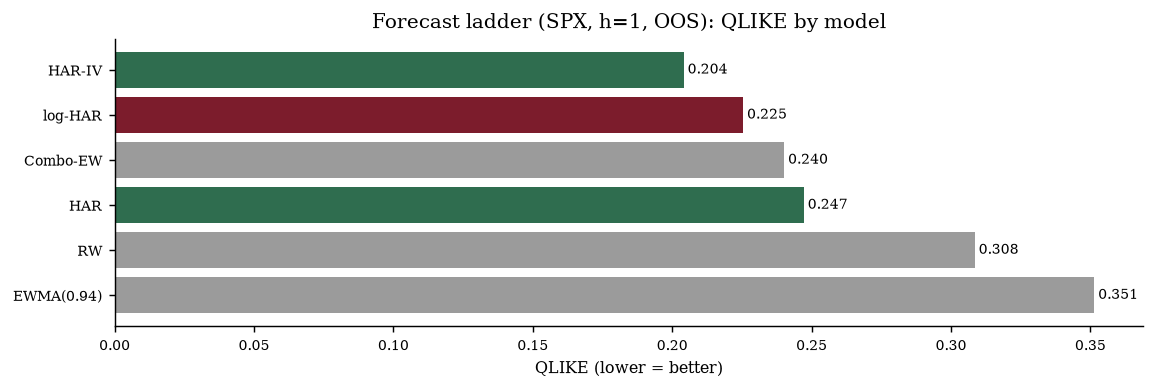
\includegraphics[width=\linewidth]{04_forecast_ladder.png}\\[1ex]
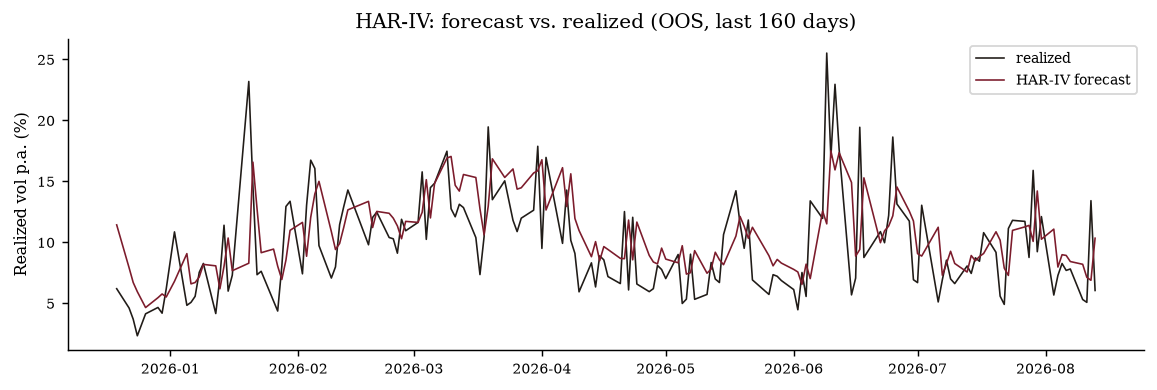
\includegraphics[width=\linewidth]{06_forecast_vs_actual.png}
\caption{Top: QLIKE by model (the level-target LHAR/HARQ/HAR-CJ variants are fit artifacts and are
omitted). Bottom: HAR-IV one-day-ahead forecasts tracking realized volatility.}
\label{fig:ladder}
\end{figure}

For the sizing rule we deliberately use log-HAR, not the best model: it is the simplest member of the
winning family, needs no auxiliary series at forecast time, and avoids stacking a second selection
layer on the strategy.

%============================ IV. LAG DIAGNOSTICS ============================
\section{Lag Diagnostics: What ``the Forecast Lags'' Really Means}

A recurring visual impression --- that the forecast ``lags'' realized volatility --- resolves into
two very different things, only one of which is a defect. Table~2 measures forecast
quality beyond the mean loss.

\begin{table}[t]\centering
\textbf{Table 2. Forecast quality beyond average loss --- out-of-sample HAR family}
\tnote{MZ slope: Mincer-Zarnowitz regression $\text{realized}\sim a+b\cdot\text{forecast}$ (1~=~calibrated
slope). The joint $a=0,\,b=1$ unbiasedness test is not rejected for HAR-IV (HAC $F$~$p=0.53$). Error
AC(1): lag-1 autocorrelation of log errors ($\approx0$~=~no exploitable linear lag-1 structure).
corr($t$)\,/\,corr($t{-}1$): correlation of the forecast with same-day versus previous-day realized
volatility. spike$\times$: mean realized\,/\,forecast on the top-decile up-jump days --- these days
are selected on the realized outcome, so a ratio $>1$ is partly mechanical (regression to the mean
under a right-skewed conditional law); the informative content is the ordering across models under a
common selection, not the absolute level.}
\begin{spacing}{1.0}
\begin{tabular}{lrrrrr}
\toprule
Model & MZ slope & err AC(1) & corr($t$) & corr($t{-}1$) & spike$\times$ \\
\midrule
Random walk           & 0.70 & $-0.329$ & 0.779 & 1.000 & 3.98 \\
log-HAR               & 1.07 & $-0.008$ & 0.800 & 0.964 & 2.73 \\
HAR-IV                & 1.02 & $-0.021$ & 0.815 & 0.961 & 2.54 \\
C2 (rich + IV-slope)  & 0.83 & $-0.029$ & 0.828 & 0.946 & 2.54 \\
\bottomrule
\end{tabular}
\end{spacing}
\label{tab:lag}
\end{table}

\emph{On the average day the forecast does not lag in any harmful sense.} The Mincer-Zarnowitz slope
is $\approx1$ (HAR-IV~1.016; the joint $a=0,\,b=1$ unbiasedness test is not rejected, HAC $F$~$p=0.53$)
and the error autocorrelation is $\approx0$ ($-0.02$): no systematic, exploitable lag-1 trailing
error. Much of what looks ``smoothed/late'' on a chart is correct behaviour --- the forecast
deliberately does not chase daily noise (five-minute RV is itself a noisy proxy of latent
volatility). The random walk, by contrast, is visibly damped (slope~0.70) with strongly negatively
autocorrelated errors ($-0.33$): it over-reacts and reverts.

\emph{The phase is ``yesterday-heavy,'' but mostly intrinsically.} HAR-IV correlates 0.96 with
yesterday's realized volatility and 0.82 with the day it forecasts --- the visible lag. This is
largely unavoidable: realized volatility is highly persistent, so forecasting a slow process is
forecasting something close to yesterday. Leading information moves the phase measurably forward ---
the rich~+~slope model has the highest same-day correlation (0.83) and the least dependence on
yesterday (0.95) --- but only at the margin.

\emph{The expensive lag is the spikes --- and we identify how much of it is real.} On the worst
$10\,\%$ up-jump days realized volatility averages $2.5\times$ the forecast (HAR-IV $2.54\times$; the
random walk $3.98\times$). This is the bulge the eye sees --- but the absolute ratio overstates the
defect, because conditioning on the realized jump forces an excess above one even for a perfect
forecaster. We separate the two. \emph{The mechanical floor:} treating the HAR-IV forecast as the
true conditional mean and drawing realized RV from the implied lognormal, a perfect forecaster
mechanically produces spike$\times = 1.90$ $[95\,\%\ 1.80,\,2.01]$ --- about three-quarters of the
observed 2.54. \emph{A genuine residual:} the observed 2.54 lies above that floor with $P<0.001$
(excess $+0.64$): there \emph{is} real under-reaction to shocks the model cannot anticipate.
\emph{Otherwise the forecast is well calibrated:} binned by \emph{forecast} decile (not outcome),
mean-realized\,/\,mean-forecast is $\approx1.0$ in every bin including the highest (1.08), and
realized exceeds the 90th predictive percentile on $9.8\,\%$ of days ($\approx$ the nominal
$10\,\%$). The reading: on the days the model itself calls high-vol it is right; the residual miss is
confined to the outcome-selected shock days, where features and implied vol shrink it (RW $3.98\to$
log-HAR $2.73\to$ HAR-IV~$2.54$) but a floor remains.

\begin{figure}[t]\centering
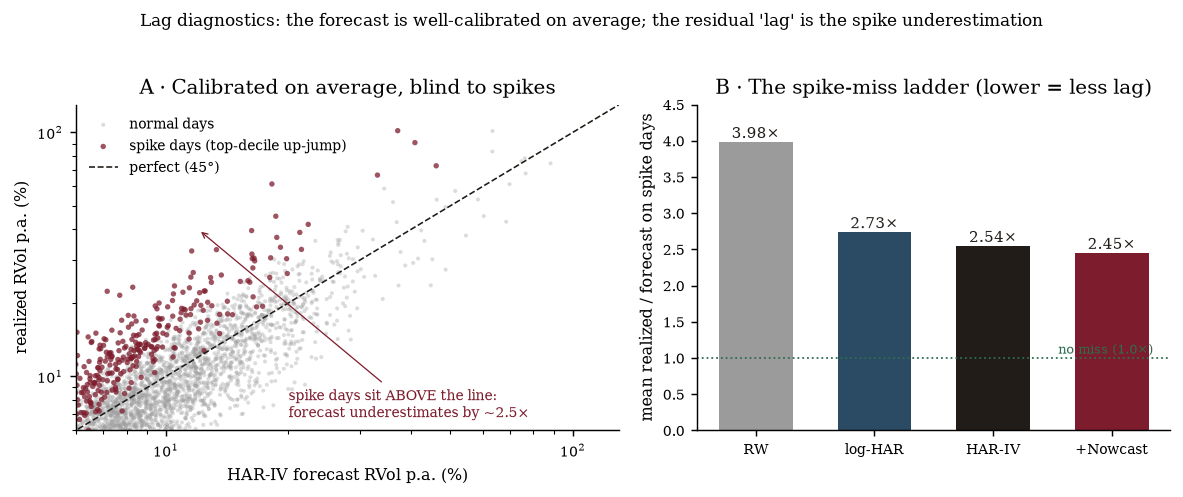
\includegraphics[width=\linewidth]{18_lag_spike.png}
\caption{(A)~HAR-IV forecast versus realized RVol: well calibrated across the bulk, but the
top-decile up-jump days (red) sit above the $45^\circ$ line --- systematically underestimated.
(B)~The spike-miss shrinks with better information (features, implied vol, an intraday nowcast) but
not to one.}
\label{fig:lagspike}
\end{figure}

\emph{Can the spikes be nowcast away?} We test the two same-day channels the data allow, incrementally
on HAR-IV (nested Clark-West), moving the forecast origin from the previous close to the morning of
day~$t$ (Table~3). Two honest findings. First, the overnight gap is nearly useless
day-ahead and only a small, non-significant help same-day ($-1.3\,\%$, $p\approx0.18$), and it does
not move the spike miss ($2.54\to2.49$): the largest RTH spikes are not gap-driven but form inside the
session. Second, intraday ``RV-so-far'' is the strongest single lever we found --- the first hour
lowers QLIKE by $4.8\,\%$ ($p=0.089$), roughly three times the overnight nowcast --- yet it still only
trims the spike miss to $2.45\times$, because on the spike days the first hour is only mildly elevated
(median morning-RV percentile 0.59). The worst spikes are realized after the first hour, so not even a
same-day nowcast sees them coming. None of these channels clears the multiple-testing bar; they are
reported as the honest ceiling of what these data support.

\begin{table}[t]\centering
\textbf{Table 3. Same-day information versus day-ahead (incremental on HAR-IV)}
\tnote{``RV-so-far'' is the realized variance of the first 30/60 one-minute bars of day~$t$, known by
10:00/10:30; the target is the full-session five-minute RV of the same day. All leakage-free. None
clears the Bonferroni threshold ($k=5$ tested, $0.05/5=0.010$). CW~$p$: nested Clark-West.}
\begin{spacing}{1.0}
\begin{tabular}{lrrrr}
\toprule
Added predictor (origin) & QLIKE & $\Delta$QLIKE & CW $p$ & spike$\times$ \\
\midrule
HAR-IV baseline (prev.\ close)          & 0.2041 & ---      & ---   & 2.54 \\
$+$ overnight gap (day-ahead)           & 0.2037 & $-0.2\,\%$ & 0.10 & 2.52 \\
$+$ $|$overnight gap$|$ (same-day)      & 0.2015 & $-1.3\,\%$ & 0.18 & 2.49 \\
$+$ RV-so-far 30\,min (nowcast)         & 0.1964 & $-3.7\,\%$ & 0.11 & 2.47 \\
$+$ RV-so-far 60\,min (nowcast)         & 0.1942 & $\mathbf{-4.8\,\%}$ & 0.09 & 2.45 \\
$+$ RV-so-far 60\,min $+$ $|$gap$|$     & 0.1940 & $-5.0\,\%$ & 0.07 & 2.43 \\
\bottomrule
\end{tabular}
\end{spacing}
\label{tab:nowcast}
\end{table}

This is \emph{consistent with} the strategy result rather than a proof of it. A volatility forecast
used to size risk must be right precisely on the days that matter --- the spikes --- and there the
miss is largest and does not vanish with more history, the overnight gap, or a morning nowcast; a
risk measure that under-reacts on the worst day de-risks a day late, after the drawdown is under way.
The visible ``lag'' and the null trading result plausibly share this mechanism --- but the trading
null already has three independent, better-identified causes (Sections~VI--VII), so we offer the
spike-miss as a coherent narrative, not a fourth proof. The \emph{target} matters too: RTH-only RV
discards the overnight component --- a median $6.8\,\%$ but a mean $15.7\,\%$ of total daily variance,
exceeding $30\,\%$ on a fifth of days --- so for a genuine total-risk objective the defensible fix is
to move overnight into the target ($\mathrm{RV}_{\text{total}}=\text{gap}^2+\text{RTH-RV}$) rather
than to use it as a feature.

%============================ V. STRATEGY + PROTOCOL ============================
\section{Strategy Design and Validation Protocol}

\emph{S1 --- Volatility-managed exposure (VMG).} $w(t)=\min(\tau(t{-}1)/\hat\sigma(t),\,c)$, where
$\tau$ is the trailing 63-day mean realized volatility, $\hat\sigma$ the log-HAR one-day-ahead
volatility forecast (information $\le t{-}1$), and $c$ the leverage cap. Net return
$w\cdot r-1\text{bp}\cdot|\Delta w|$. High-volatility days do not carry proportionally higher expected
returns,\cf{Moreira \& Muir (2017).} so scaling down ahead of turbulence harvests the premium with
fewer of the worst days. Walk-forward re-selects (target window, cap) annually from
$\{21,42,63,126\}\times\{1.5,2,3\}$.

\emph{S2 --- VIX term-structure conditioning (VIXTS).} Exposure keyed to VXV/VIX: full in contango
(the volatility risk premium),\cf{Whaley (2009); Simon \& Campasano (2014).} reduced in backwardation.
Unlike S1 the signal is implied, so it complements the realized channel. Supporting sleeves are TSMOM
(long/flat, vol-targeted; the short leg is rejected decisively) and short-term reversal. A
single-market combination weights these sleeve return streams inversely to their trailing 63-day
volatility.

\emph{Protocol.} (1)~\emph{Pre-registration}\cf{The campaign protocol is
\texttt{PREREGISTRATION-EN.md} (QR006); the headline forecasting claim is pre-registered separately
in \texttt{PREREGISTRATION-FORECAST-EN.md} (QR002). Both are released.}\emph{:} six hypothesis families with null and expected effect;
the complete grids; costs (1/2/5\,bp); the out-of-sample split; the composite ranking score
$0.30\cdot\text{Sortino}+0.25\cdot\text{Calmar}+0.20\cdot\text{Sharpe}+0.15\cdot\text{YearConsistency}+0.10\cdot\min(\text{PF}{-}1,1)\cdot5$;
and --- decisive here --- the disqualification rules: DSR $<0.5$, PBO $>0.7$, single-market-only
effect, or a synthetic-data-only basis. Nothing was added after the first result. (2)~\emph{Walk-forward:}
anchored five-year train, one-year test, stepped annually; only concatenated test segments are ranked
or combined. (3)~\emph{Multiple testing:} deflated Sharpe ratio\cf{Bailey \& L\'opez de Prado (2014).}
against the expected maximum of $n=73$ SPX-only trials; PBO via combinatorially symmetric
cross-validation;\cf{Bailey, Borwein, L\'opez de Prado \& Zhu (2017).} block-bootstrap Sharpe intervals
(21-day blocks). (4)~\emph{Distributional risk:} fixed 21-day block-bootstrap Monte-Carlo ($5{,}000$
paths, seed~42).

\begin{figure}[t]\centering
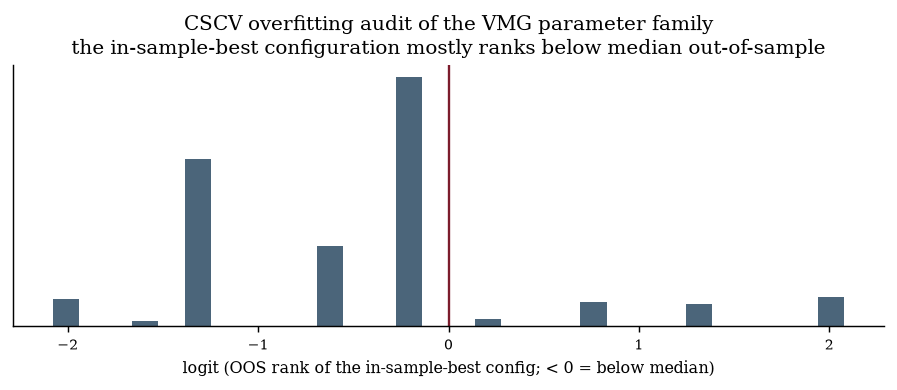
\includegraphics[width=0.85\linewidth]{13_pbo.png}
\caption{CSCV overfitting audit (illustrative $2\times2\times2$ VMG grid). In the full campaign the
VMG parameter family has PBO~$=0.79$ (HAR-IV; $0.75$ for log-HAR) and the combination universe PBO~$=0.84$ --- both above the
$0.7$ disqualification gate; the in-sample-best configuration mostly ranks below median
out-of-sample.}
\label{fig:pbo}
\end{figure}

%============================ VI. RESULTS ============================
\section{Results: the Disqualified Campaign}

Walk-forward parameter selection resolves the well-known overfitting paradox of volatility
management at the family level: the fixed in-sample-best VMG parametrization is overfit
(PBO~$=0.79$ for HAR-IV, $0.75$ for log-HAR on SPX; \texttt{thesis\_validation.csv} --- though the same file reports PBO~$=0.365$ on NDX, so this overfitting flag is market-specific, a caveat the SPX-only headline should carry),\cf{Consistent with Cederburg, O'Doherty, Wang \& Yan (2020).} yet the family, honestly re-selected,
delivers a positive walk-forward Sharpe. The combination then looks good on paper
(Table~4).

\begin{table}[t]\centering
\textbf{Table 4. The campaign combination (net, out-of-sample, SPX)}
\tnote{The best walk-forward volatility-managed / VIX-term-structure combination against single-sleeve
VMG and buy-and-hold. Sharpe intervals are 21-day block-bootstrap 95\,\% intervals. P(drawdown~$>20\,\%$)
is from the fixed-block bootstrap Monte-Carlo (only the forecasting MCS uses a stationary bootstrap).}
\begin{spacing}{1.0}
\begin{tabular}{lrrr}
\toprule
Metric & Best combo & VMG (single) & Buy \& Hold \\
\midrule
Sharpe $[95\,\%\text{ CI}]$      & \textbf{0.96} $[0.44,1.46]$ & 0.95 & 0.83 $[0.28,1.34]$ \\
Maximum drawdown                 & $\mathbf{-9.9\,\%}$ & $-25.1\,\%$ & $-34.0\,\%$ \\
Calmar                           & 0.62 & 0.57 & 0.39 \\
Deflated Sharpe ($n=73$)         & 0.99 & 0.97 & 0.96 \\
MC P(drawdown $>20\,\%$)         & $3.5\,\%$ & $72\,\%$ & $91\,\%$ \\
\bottomrule
\end{tabular}
\end{spacing}
\label{tab:campaign}
\end{table}

But the campaign fails its own pre-registered gates. \emph{Single-market effect $\to$ disqualified:}
by construction every SPX-only combination is a single-market result, and the fixed rules disqualify
single-market-only effects. \emph{PBO $=0.84\to$ disqualified:} the probability that the selection is
overfit is 0.84, far above the 0.7 gate. \emph{No significant Sharpe advantage:} $\Delta$Sharpe over
buy-and-hold is $+0.13$, but the 95\,\% Sharpe intervals overlap heavily ($[0.44,1.46]$ versus
$[0.28,1.34]$). \emph{The clean tail is mostly a volatility artifact:} the combination runs at
$\approx6.5\,\%$ volatility versus $\approx17\,\%$ for buy-and-hold; normalized to a common risk level
the drawdown advantage shrinks toward parity, and single-market VMG alone matches or beats the
combination on vol-matched Calmar. We therefore report no tradeable edge.

\emph{Cost stress and the graveyard.} VMG and VIXTS survive five basis points --- though VIXTS survives the \emph{cost} stress, not its own hypothesis: the pre-registered Q015 (VIX-term-structure sizing improving Calmar by $+0.05$ to $+0.15$) reaches only $\Delta$Calmar~$\approx+0.023$ at its best grid point, with four of six grid points negative, so it misses its pre-registered band and is recorded \emph{not supported}; and Q012 (TSMOM, correlation $<0.5$ to VMG) measures $0.751$, violating its own condition. The cost-fragile
families die where they should --- overnight carry collapses to Sharpe $-2.38$ at five basis points
despite a real gross anomaly ($+7.3\,\%$/yr overnight versus $+6.4\,\%$ intraday). Reported failures in
full: long/short momentum ($-52\,\%$ SPX drawdown; the $-68\,\%$ sometimes quoted was the DAX sleeve in the earlier cross-market version), turn-of-month (a single-market artifact), net overnight
carry, and a six-test mechanism battery in which only HAR-IV (implied volatility helps, $p=0.019$)
carried evidence; the other five were null or weak.

\emph{Why the trading result is null --- and why that is the point.} The volatility-managed idea is
real (it survives walk-forward at the family level); the tradeable claim is not established, for three
independent reasons that all point the same way: on a single market the effect is disqualified by the
ex-ante rule; the selection among combinations is overfit (PBO~0.84); and the return-metric advantage
is inside the bootstrap noise while the risk-metric advantage is largely a volatility level, not
diversification. Any one would be enough. A fourth, mechanistic reading is consistent with them (though
less cleanly identified, Section~IV): the sizing forecast under-reacts most on exactly the spike days a
risk overlay exists to catch, so it de-risks a day late. A paper that buried these behind a 0.96 Sharpe
would be exactly the kind of result the replication literature warns about;\cf{White (2000); Harvey,
Liu \& Zhu (2016); Bailey, Borwein, L\'opez de Prado \& Zhu (2014).} reporting them is the contribution.

%============================ VII. IMPLEMENTATION ============================
\section{Implementation and Costs}

The backtest is on the S\&P~500 price index, which is not directly tradeable; a live implementation
would use ES/MES futures, whose all-in cost (bid/ask, roll, slippage in volatility spikes) exceeds the
one basis point modeled here --- the two/five basis-point stress is the honest bracket, and the
overnight-carry collapse shows the strategies live close to their cost breakeven. Signals are formed
at or near the close (a fifteen-minute approximation versus the exact close used in the backtest,
documented as a gap), executed market-on-close, with profit and loss aligned close-to-close. None of
this rescues the null result; it is stated so the reader can see the execution assumptions rather than
infer them.

%============================ VIII. CRITICAL ASSESSMENT ============================
\section{Critical Assessment}

\emph{(1)~Forecasting is mostly replication.} log-HAR $\succ$ RW and HAR-IV are known; the
contribution there is a clean, leakage-tested, single-market replication with honest tests. The one
genuine increment is the loss-matched Gamma-GLM with the VIX term-structure slope (Section~III\,f) ---
real by our gates, but unconfirmed absent a live log. \emph{(2)~The strategy is beta management at
best,} and here not even that survives selection: no short book, no market-neutral source, and on one
market the diversification argument is thin. \emph{(3)~Statistical honesty about ranks and
differences:} the deflated Sharpe of the leaders is high only because restricting to SPX shrinks the
trial count ($227\to73$); we report this openly and rest the conclusion on the PBO/single-market
disqualification, not on the flattering DSR. \emph{(4)~The decisive scenarios are out of sample:} no
2008 inside the OOS window, no slow-grind bear anywhere in the data. \emph{(5)~No live track record:}
a pre-registered, micro-size prediction log is the only route from \texttt{testing} to evidence; every
number here deserves a 30--50\,\% haircut until it exists. \emph{(6)~The lag/spike diagnostic is where
method meets substance:} decomposing the ``forecast lag'' into a calibrated mean and a residual
spike-miss, and relating that spike-miss to why the sizing strategy struggles, is the paper's freshest
piece of reasoning --- with the caveat that the spike ratio conditions on the outcome and so is a
coherent narrative, not a clean identification. On our own honest ledger: methodology strong,
execution solid, novelty deliberately modest.

%============================ IX. CONCLUSION ============================
\section{Conclusion}

On 21 years of intraday S\&P~500 data, evaluated under a pre-registered, walk-forward,
multiple-testing-corrected protocol: (1)~realized volatility is forecastable --- log-HAR beats the
random walk, implied volatility adds information, and the gain over HAR comes from features rather than
regularization or nonlinearity; (2)~the corresponding volatility-managed / VIX sizing strategy, however
good it looks, is disqualified by the study's own rules and is reported as a null. The failures are
reported with equal weight. The publishable, reproducible contribution is the forecasting result plus
the validation methodology --- and the demonstration that a disciplined protocol will, and should, kill
one's favourite backtest.

\emph{Future work,} in order of value: (1)~a live prediction log, the only route from \texttt{testing}
to \texttt{supported}, paired with a real ES/MES execution and option-chain cost model; (2)~deciding the
question up front --- a forecasting paper or a strategy paper, the latter requiring multi-asset data
from the outset because the single-market disqualification cannot be satisfied on the S\&P complex
alone; (3)~coupling loss and estimator throughout, making the QLIKE-native Gamma-GLM the default fitter;
(4)~exploiting the one-minute data already in hand --- noise-robust estimators, overnight variance as a
target component, and the intraday nowcast track; (5)~acquiring horizon-matched leading inputs
(VIX9D, VVIX, SKEW); (6)~extending the Model Confidence Set to the full feature/ML-inclusive ladder,
adding rolling-origin cross-validation, block-bootstrap confidence intervals on loss differences, and a
de-risk-before-drawdown hit-rate as a first-class outcome; and (7)~modelling the distribution, not just
the point, and coupling it to sizing.

%============================ REFERENCES ============================
\section*{References}
\addcontentsline{toc}{section}{References}
\begin{spacing}{1.0}
\begin{list}{}{\leftmargin=1.5em \itemindent=-1.5em \itemsep=0.5em}

\item Andersen, Torben G., Tim Bollerslev, Francis X.\ Diebold, and Paul Labys, 2003, Modeling and
forecasting realized volatility, \emph{Econometrica} 71, 579--625.

\item Bailey, David H., and Marcos L\'opez de Prado, 2014, The deflated Sharpe ratio: Correcting for
selection bias, backtest overfitting, and non-normality, \emph{Journal of Portfolio Management} 40,
94--107.

\item Bailey, David H., Jonathan M.\ Borwein, Marcos L\'opez de Prado, and Qiji J.\ Zhu, 2014,
Pseudo-mathematics and financial charlatanism, \emph{Notices of the AMS} 61, 458--471.

\item Bailey, David H., Jonathan M.\ Borwein, Marcos L\'opez de Prado, and Qiji J.\ Zhu, 2017, The
probability of backtest overfitting, \emph{Journal of Computational Finance} 20, 39--69.

\item Barndorff-Nielsen, Ole E., and Neil Shephard, 2004, Power and bipower variation with stochastic
volatility and jumps, \emph{Journal of Financial Econometrics} 2, 1--37.

\item Bollerslev, Tim, 1986, Generalized autoregressive conditional heteroskedasticity, \emph{Journal
of Econometrics} 31, 307--327.

\item Bollerslev, Tim, Andrew J.\ Patton, and Rogier Quaedvlieg, 2016, Exploiting the errors: A simple
approach for improved volatility forecasting, \emph{Journal of Econometrics} 192, 1--18.

\item Cederburg, Scott, Michael S.\ O'Doherty, Feifei Wang, and Xuemin Sterling Yan, 2020, On the
performance of volatility-managed portfolios, \emph{Journal of Financial Economics} 138, 95--117.

\item Clark, Todd E., and Kenneth D.\ West, 2007, Approximately normal tests for equal predictive
accuracy in nested models, \emph{Journal of Econometrics} 138, 291--311.

\item Corsi, Fulvio, 2009, A simple approximate long-memory model of realized volatility, \emph{Journal
of Financial Econometrics} 7, 174--196.

\item Diebold, Francis X., and Roberto S.\ Mariano, 1995, Comparing predictive accuracy, \emph{Journal
of Business and Economic Statistics} 13, 253--263.

\item Hansen, Peter R., Asger Lunde, and James M.\ Nason, 2011, The model confidence set,
\emph{Econometrica} 79, 453--497.

\item Harvey, Campbell R., Yan Liu, and Heqing Zhu, 2016, \ldots and the cross-section of expected
returns, \emph{Review of Financial Studies} 29, 5--68.

\item Liu, Lily Y., Andrew J.\ Patton, and Kevin Sheppard, 2015, Does anything beat 5-minute RV? A
comparison of realized measures across multiple asset classes, \emph{Journal of Econometrics} 187,
293--311.

\item Moreira, Alan, and Tyler Muir, 2017, Volatility-managed portfolios, \emph{Journal of Finance} 72,
1611--1644.

\item Patton, Andrew J., 2011, Volatility forecast comparison using imperfect volatility proxies,
\emph{Journal of Econometrics} 160, 246--256.

\item Simon, David P., and Jim Campasano, 2014, The VIX futures basis: Evidence and trading strategies,
\emph{Journal of Derivatives} 21, 54--69.

\item Whaley, Robert E., 2009, Understanding the VIX, \emph{Journal of Portfolio Management} 35, 98--105.

\item White, Halbert, 2000, A reality check for data snooping, \emph{Econometrica} 68, 1097--1126.

\end{list}
\end{spacing}

\vfill
\sloppy\noindent\small\emph{Working paper v1.0, \today. Reproduction: the two pre-registration
protocols (\texttt{PREREGISTRATION-FORECAST-EN.md} for the forecasting claim,
\texttt{PREREGISTRATION-EN.md} for the campaign), all grids and the SPX
candidate table are distributed with the code; forecasting via \texttt{analyze.py}, \texttt{ml\_models.py},
\texttt{paper\_fills\_mcs.py} (Model Confidence Set) and the diagnostics \texttt{rv\_lag\_diag.py},
\texttt{rv\_spike\_ident.py}, \texttt{rv\_overnight.py}, \texttt{rv\_nowcast.py}, \texttt{rv\_improve.py};
strategy via \texttt{strategy\_lab.py}, \texttt{walkforward.py}, \texttt{portfolio\_combos.py},
\texttt{sensitivity.py}. Smoke test without licensed data: \texttt{python run.py} (synthetic, seed~42).
Random seeds fixed (42); data fingerprints in \texttt{data/data\_manifest.csv}. Comments welcome via the
repository issue tracker.}

\end{document}
